\begin{figure}
  \ContinuedFloat*
  \begin{tabular}[t]{c c}
    \begin{minipage}{0.5\textwidth}
      \begin{Verbatim}[mathescape,commandchars=\\\{\}]
\textbf{let} s = stim 2 \textbf{in}
  \textbf{let} p = pop 2 \textbf{in}
      $\otimes$ s p 1
      \end{Verbatim}
    \end{minipage} & \begin{minipage}{0.5\textwidth}
      \includegraphics[width=\textwidth]{chapters/volr/example2.pdf}
    \end{minipage}

  \end{tabular}
  \caption{A textual and visual example of a network
    with a stimulus containing two channels. 
    The stimulus is fully connected to a population with an excitatory
    weight of 1. Each node represents a single neuron.}
  \label{fig:volr-example1}
\end{figure}

\begin{figure}
  \ContinuedFloat
  \begin{tabular}[t]{c c}
    \begin{minipage}{0.5\textwidth}
      \begin{Verbatim}[mathescape,commandchars=\\\{\}]
\textbf{let} s1 = stim 1 \textbf{in}
  \textbf{let} s2 = stim 1 \textbf{in}
    \textbf{let} p = pop 1 \textbf{in}
      $\ominus$ s1 p 1 \textbf{,} $\ominus$ s2 p -1
      \end{Verbatim}
    \end{minipage} & \begin{minipage}{0.5\textwidth}
      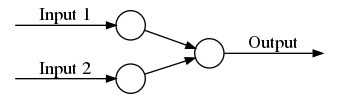
\includegraphics[width=\textwidth]{chapters/volr/example1.pdf}
    \end{minipage}
  \end{tabular}
  \caption{An illustration of a simple network that can solve a
    T-maze task. A single population (\texttt{\textbf{p}}) is 
    excited and inhibited by two different stimulus channels, initialised
    to the value of 1 and -1 respectively.}
\end{figure}

\begin{figure}
  \ContinuedFloat
  \begin{tabular}[t]{c c}
    \begin{minipage}{0.4\textwidth}
      \begin{Verbatim}[mathescape,commandchars=\\\{\}]
\textbf{let} s = stim 256 \textbf{in}
  \textbf{let} p = pop 256 \textbf{in}
    \textbf{let} o = pop 10 \textbf{in}
      $\ominus$ s p 1
      $\otimes$ p o 1
      \end{Verbatim}
    \end{minipage} & \begin{minipage}{0.6\textwidth}
      \includegraphics[width=\textwidth]{chapters/volr/example3.pdf}
    \end{minipage}
  \end{tabular}
  \caption{A more advanced example, that can process the MNIST dataset
    as 16x16 pixel images. 
    The nodes are no longer single neurons, but populations of neurons,
    where the input (16x16 = 256) is connected one-to-one
    with the first population (256), which is connected all-to-all to the 
    output population (9).}
\end{figure}

\begin{figure}
  \ContinuedFloat
  \begin{tabular}[t]{c c}
    \begin{minipage}{0.45\textwidth}
      \begin{Verbatim}[mathescape,commandchars=\\\{\}]
\textbf{let} s = stim 2 \textbf{in}
\textbf{let} l$_1$ = pop 4 \textbf{in} $\otimes$ s l$_1$ 1
\textbf{let} l$_2$ = pop 4 \textbf{in} $\otimes$ s l$_1$ 1

\textbf{let} o = pop 1 \textbf{in} 
  $\otimes$ l$_1$ o 1 \textbf{,} $\otimes$ l$_2$ o -1
      \end{Verbatim}
    \end{minipage} & \begin{minipage}{0.55\textwidth}
       \includegraphics[width=\textwidth]{chapters/volr/example4.pdf}
    \end{minipage}
  \end{tabular}
   \caption{An example where a two-dimensional input is split into
     two nodes and later merged---excitatorily and inhibitorily---into 
     a node of a single neuron.}
  \label{fig:volr-example}
\end{figure}
